\documentclass[letterpaper,12pt]{exam}
\usepackage[utf8x]{inputenc}
\usepackage{amsmath,anysize,graphicx,siunitx}
\usepackage{booktabs}
\usepackage[colorlinks, bookmarks, urlcolor=cyan, linkcolor=black]{hyperref}
\usepackage{caption, subcaption}
%\usepackage{titlesec, titletoc}
\usepackage{python-commands}
\marginsize{1in}{1in}{1in}{0.5in}

\sisetup{per-mode=symbol}
\graphicspath{ {Images/} }
\captionsetup{margin=2cm}

%\titleformat{\section}{\normalfont\Large\bfseries}
%{Milestone\ \thesection:}{1.3ex plus .2ex}{}
%\addtocounter{section}{0} %Starting here at Milestone 1

\newcommand{\class}{CS 151}
\newcommand{\due}{Fri, February 17, 2023}
\newcommand{\project}{Wordle}

% Setting up headers and footers
\pagestyle{headandfoot}
\firstpageheader{}{\Large\textbf{Project 1: \project}}{}
\firstpageheadrule
\firstpagefootrule
\firstpagefooter{Due \due}{}{\thepage}
\runningheadrule
\runningheader{}{\project}{}
\runningfooter{\hyperlink{toc}{Table of Contents}}{\class}{\thepage}
\runningfootrule

\usepackage{pgfornament}

\newcommand{\sectionlinetwo}[2]{%
  \nointerlineskip \vspace{.5\baselineskip}\hspace{\fill}
  {\resizebox{0.5\linewidth}{1.0ex}
    {\pgfornament[color = #1]{#2}
    }}%
    \hspace{\fill}
    \par\nointerlineskip \vspace{.5\baselineskip}
  }
\setcounter{secnumdepth}{0}

\definecolor{CORRECT}{HTML}{66BB66}
\definecolor{PRESENT}{HTML}{CCBB66}
\definecolor{MISSING}{HTML}{999999}

%\printanswers

\begin{document}
Welcome to the first project of CS 151! This project is designed to help you practice working with strings in the context of an engaging application: the Wordle game initially developed by Josh Wardle, now available on the \emph{New York Times} website. Given Wordle's enormous popularity, we thought it would be fun to give you a chance to implement the game!

As per usual, you will submit this through GitHub Classroom, and you can find the link to accept the project and download the initial template files \href{https://classroom.github.com/a/-0Ri2Gix}{\textbf{here}}. To help you navigate the project, I've included a table of contents below, but I highly recommend you read everything as you work through the project. If you want to check yourself, a working demonstration of the final program is available \href{https://willamette.edu/~esroberts/NiftyAssignments-2022/demos/Wordle.html}{here}.

\addtocontents{toc}{\protect\hypertarget{toc}{}}
\tableofcontents
\vspace{8mm}
\sectionlinetwo{black}{86}

\section{The Starting Template}
The good news is that you don't have to implement the Wordle project entirely from scratch. The starting repository already include the following files:
\begin{center}
	\begin{tabular}{lp{10cm}}
		\toprule
		\pyi{Wordle.py} & The starter file for the project, which uses the \pyi{WordleGraphics} module to display the board. \\
		\pyi{WordleGraphics.py} & This module exports the \pyi{WordleGWindow} type, which is responsible for the graphics, along with several useful constants. \\
		\pyi{english.py} & This module exports the constant \pyi{ENGLISH_WORDS}, and a function \pyi{is_english_word(s)} that checks whether \pyi{s} is a valid English word. Especially for this project, it also exports the constant \pyi{CAPITAL_ENGLISH_WORDS}, which are uppercase versions of all the English words. This is convenient since the Wordle graphics like to work with capital letters.\\
		\bottomrule
	\end{tabular}
\end{center}

Unless you are implementing extensions, the only file you need to change is \pyi{Wordle.py}, which imports the resources it needs from the other modules. The starting version of \pyi{Wordle.py} is included in the starting resources, but is included here in Figure~\ref{fig:wordlestart} below for later reference.

\begin{figure}[!hb]
	\centering\scriptsize
	\lstinputlisting[style=basic,numbers=left]{./Wordle.py}
	\caption{The starting state of \pyi{Wordle.py}. Of particular importance is line 21, where an instance of the \pyi{WordleGWindow} data type is stored in the variable \pyi{gw}. This is the variable you will use throughout the rest of the program when wanting to interact with the \pyi{WordleGWindow}.}
	\label{fig:wordlestart}
\end{figure}

When you download the initial repository, a lot of the code is already running because we have implemented the graphics for you. Running \pyi{Wordle.py} creates a window, draws the letter boxes, and creates the keyboard at the bottom of the window. You can even type letters either by hitting keys on the keyboard or clicking the key on the screen, just as you can when you are playing the online version. Figure~\ref{fig:wordle_starts} shows both the initial screen and the screen you get after typing in the five letters of the useful starting work \texttt{RATES}, which includes five of the most common letters.

Unfortunately, that is all the program does at the moment. It doesn't actually let you play the Wordle game. That's your job! But first, it is worth spending a bit of time reviewing the rules of Wordle, in case you've somehow managed to miss the craze.

\begin{figure}[!ht]
	\centering
	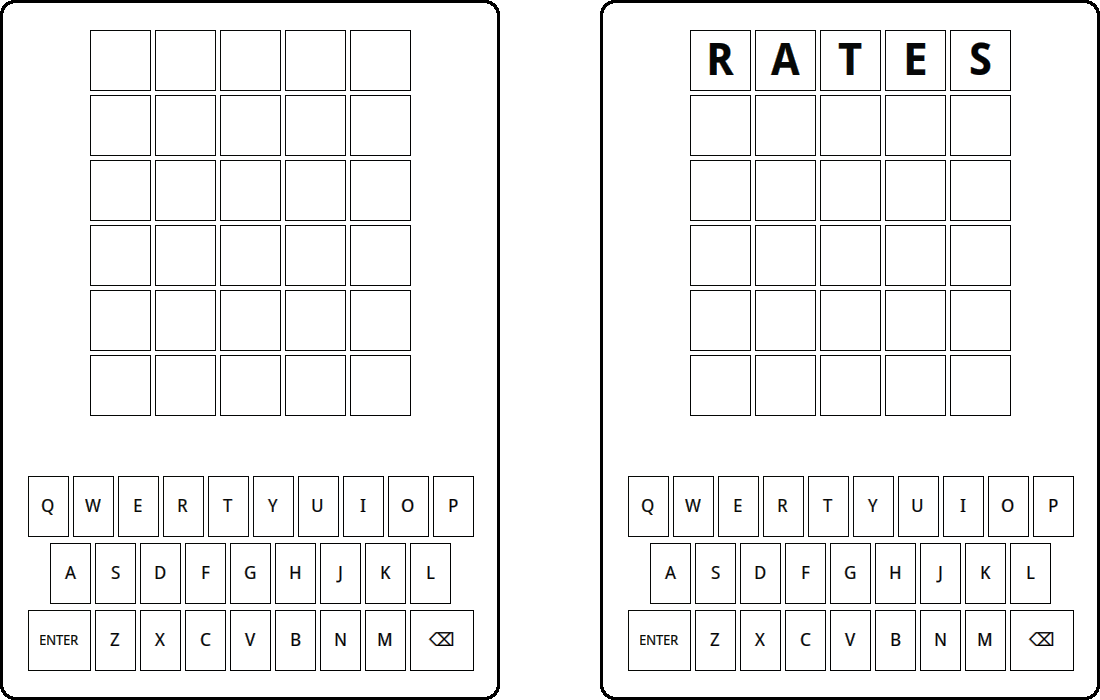
\includegraphics[width=0.7\linewidth]{./initial.png}
	\caption{The current state of the window both initially (left), and then after typing in the letters \texttt{RATES} (right).}
	\label{fig:wordle_starts}
\end{figure}

\section{Playing Wordle}
The object of the Wordle puzzle is to figure out the hidden word for the day using no more than six guesses. When you type in a word and then hit the \texttt{RETURN} or \texttt{ENTER} key, the game gives you information about how close your guess is by coloring the background of the letters. For every letter in your guess that is in its correct position, Wordle colors the background of that letter a light shade of green, indicated in your program by the constant \pyi{CORRECT_COLOR}. For every letter that appears in the word but is not in the correct position, Wordle colors the background a brownish yellow (\pyi{PRESENT_COLOR} in your program). All letters in the guess that don't appear in the word are colored a medium gray (\pyi{MISSING_COLOR} in your code).

For example, suppose that the hidden word for the day was \texttt{RELIC}, and your first guess was \texttt{RATES} as in the Figure~\ref{fig:wordle_starts} image. The \texttt{R} is in the correct position, and the word contains an \texttt{E}, but not in the position you guessed. The hidden word does not contain any of the letters \texttt{T}, \texttt{A}, and \texttt{S}. Wordle reports that information by changing the background color of the squares like this:
\begin{center}
	\begin{tikzpicture}[every node/.style={draw, minimum size=1cm, font=\bfseries\sffamily\Huge, text=white}]
		\node[fill=CORRECT](R) at (0,0) {R};
		\node[fill=MISSING, right=2pt of R](A) {A};
		\node[fill=MISSING, right=2pt of A](T) {T};
		\node[fill=PRESENT, right=2pt of T](E) {E};
		\node[fill=MISSING, right=2pt of E](S) {S};
	\end{tikzpicture}
\end{center}

Even though you know the position of the \texttt{R}, it doesn't make sense to  guess more words beginning with \texttt{R} at this point because doing so gives you no new information (assuming you are not playing in hard mode, where you are required to do so). Suppose that you tried guessing the word \texttt{LINGO}, which contains five new letters, two of which appear in the word, but none of which are correctly positioned. Wordle responds by coloring the letters in your second guess as follows:
\begin{center}
	\begin{tikzpicture}[every node/.style={draw, minimum size=1cm, font=\bfseries\sffamily\Huge, text=white}]
		\node[fill=PRESENT](1) at (0,0) {L};
		\node[fill=PRESENT, right=2pt of 1](2) {I};
		\node[fill=MISSING, right=2pt of 2](3) {N};
		\node[fill=MISSING, right=2pt of 3](4) {G};
		\node[fill=MISSING, right=2pt of 4](5) {O};
	\end{tikzpicture}
\end{center}

Putting these clues together means that you know that the word begins with an \texttt{R}, contains the letters \texttt{E}, \texttt{L}, and \texttt{I} in some order other than the one you guessed, and that the letters \texttt{A}, \texttt{T}, \texttt{S}, \texttt{N}, \texttt{G} and \texttt{O} do not appear anywhere in the word. These answers give you an enormous amount of information! If you think carefully about it, you might find the word \texttt{RELIC}, which is in fact the only English word that meets these conditions:
\begin{center}
	\begin{tikzpicture}[every node/.style={draw, minimum size=1cm, font=\bfseries\sffamily\Huge, text=white}]
		\node[fill=CORRECT](1) at (0,0) {R};
		\node[fill=CORRECT, right=2pt of 1](2) {E};
		\node[fill=CORRECT, right=2pt of 2](3) {L};
		\node[fill=CORRECT, right=2pt of 3](4) {I};
		\node[fill=CORRECT, right=2pt of 4](5) {C};
	\end{tikzpicture}
\end{center}
Done in three!

It is worth noting a few other rules and special cases. The hidden word and each of your guesses must be a real English word that is five letters long. The file \pyi{english.py} included in the repository is described in Chapter 3 of the text, and exports three resources here: the constant \pyi{ENGLISH_WORDS}, which is a list of all valid English words in lowercase (of any length, not just the five-letter ones!), a function \pyi{is_english_word(s)}, which tests whether \pyi{s} is an English word, and the constant \pyi{CAPITAL_ENGLISH_WORDS}, which is a list of all the valid English words fully capitalized (and still of any length). If you guess a word that is not in the word list, Wordle displays a message to that effect, at which point you can delete the letters you've entered and try again. Another rule is that you only get six guesses. If all the letters don't match by then, Wordle gives up on you and tells you what the hidden word was.

The most interesting special cases arise when the hidden word and the guesses contain multiple copies of the same letter. Suppose, for example, that the hidden word is \texttt{GLASS} and you for some reason guess \texttt{SASSY}. Wordle responds with the following colors:
\begin{center}
	\begin{tikzpicture}[every node/.style={draw, minimum size=1cm, font=\bfseries\sffamily\Huge, text=white}]
		\node[fill=PRESENT](1) at (0,0) {S};
		\node[fill=PRESENT, right=2pt of 1](2) {A};
		\node[fill=MISSING, right=2pt of 2](3) {S};
		\node[fill=CORRECT, right=2pt of 3](4) {S};
		\node[fill=MISSING, right=2pt of 4](5) {Y};
	\end{tikzpicture}
\end{center}
The green \texttt{S} shows that there is an \texttt{S} in the fourth position, and the yellow \texttt{S} shows that a second \texttt{S} appears somewhere else in the hidden word. The \texttt{S} in the middle of \texttt{SASSY}, however, remains gray because the hidden word does not contain three instances of the letter \texttt{S}.

\section{The WordleGraphics module}
Even though you don't have to make any changes to it or understand the details of its operation, you need to know what capabilities the \pyi{WordleGraphics} module has on offer so that you can use those facilities in your code. The most important thing to know is that this library module exports a data type called \pyi{WordleGWindow}, which implements all the graphical capabilities of the game. The methods exported by the \pyi{WordleGWindow} type are outlined below in Table~\ref{tab:gwmethods}. The right column gives a brief description of what these methods do, though more complete descriptions appear later in this guide in the description of the milestones that require them.
\begin{table}[!ht]
	\centering
	\small
	\begin{tabular}{ll}
		\toprule
		\pyi[syntax]{WordleGWindow()} & Creates and displays the graphics window \\
		\pyi[syntax]{.set_square_letter(|row|, |col|, |letter|)} & Sets the letter in the specified row and column.\\
		\pyi[syntax]{.get_square_letter(|row|, |col|)} & Returns the letter in the specified row and column. \\
		\pyi[syntax]{.add_enter_listener(|func|)} & Specifies a callback function for the \texttt{ENTER} key. \\
		\pyi[syntax]{.show_message(|msg|)} & Shows a message below the squares. \\
		\pyi[syntax]{.set_square_color(|row|, |col|, |color|)} & Sets the color of the specified square. \\
		\pyi[syntax]{.get_square_color(|row|, |col|)} & Returns the color of the specified square. \\
		\pyi[syntax]{.set_current_row(|row|)} & Sets the row in which typed characters appear. \\
		\pyi[syntax]{.get_current_row()} & Returns the current row index. \\
		\pyi[syntax]{.set_key_color(|letter|, |color|)} & Sets the color of the specified key letter. \\
		\pyi[syntax]{.get_key_color(|letter|)} & Returns the color of the specified key letter. \\
		\bottomrule
	\end{tabular}
	\caption{A listing and description of the variety of methods available to manipulate a \pyi{WordleGWindow} object. I have included the dot before each method name as a reminder that you will call these methods on the \pyi{WordleGWindow} object using the receiver syntax we discussed in class. In the starting code, that object is named \pyi{gw} and is defined on line 21. }
	\label{tab:gwmethods}
\end{table}

\section{Milestones}
Whenever you are working on a programming project of any significant size, you should never try to get the entire project running all at once (until the very end). A much more effective strategy is to define a series of milestones that allow you to complete and test the project in stages. Ideally, each milestone you choose should be a program that you can test and debug independently, even if the code you write to test a particular milestone doesn't make its way into the finished project. The advantage you get from making it possible to test each stage more than compensates for having to write a little extra code along the way. Similarly, it often makes sense to defer more of the more complex aspects of the project until after you have gotten the basic foundation working. The next few sections outline four milestones for the Wordle project that walk you through different stages of the implementation. \emph{You should get each one working before moving on to the next one.}

\subsection{Milestone 1: Pick a random word and display it}
For your first milestone, all you have to do is choose a random word from the list provided in the \pyi{english.py} module and then have that word appear in the five boxes across the first row of the window. This milestone requires fewer than ten lines of code, but requires you to understand the tools you have and start putting them to use. For example, the \pyi{WordleGWindow} type does not export any method for displaying an entire word. All you have is a method \pyi{set_square_letter} that puts one letter in a box identified by its row and column numbers. You also need to remember that \pyi{CAPITAL_ENGLISH_WORDS} contains all English words and not just the ones with five letters.

As with everything in Python, rows and columns are numbered beginning with 0, so that the top row of the window is row 0, and its column numbers range from 0 to 4. To avoid cluttering up your code with numbers that don't tell you anything about what they represent (where does 4 come from in the previous sentence, for example?), it is best to import the constants \pyi{N_ROWS} and \pyi{N_COLS} from \pyi{WordleGraphics} and use those constants wherever your code needs to know how many rows or columns exist. Not only does \pyi{N_COLS - 1} provide more insight than the number 4, but this strategy also makes it far easier to implement a SuperWordle extension with longer words or a different number of guesses.

Once you have the randomly chosen word displaying on the screen, realize that you don't really want this to happen in the actual game. After all, that would make it rather easy to guess! It highlights the fact though that often times it can be worth doing a little work that will later be unnecessary, if it helps you better understand the tools and problem-solving strategies at your disposal. In this case, you will absolutely still need the random word later, but you can remove the code to display it to the first row once you have determined that you know how to do so.

\subsection{Milestone 2: Checking for valid words}
Although the starting program allows the user to type letters into the Wordle game, nothing happens when you hit the \texttt{RETURN} key or click the \texttt{ENTER} button. The \pyi{WordleGWindow} type lets you respond to that event through the \pyi{add_enter_listener} method that works in much the same way that \pyi{add_event_listener} does in the \pyi{GWindow} object type. If you call
\begin{pythoncode}[style=syntax]
	gw.add_enter_listener(enter_action)
\end{pythoncode}
then typing \texttt{RETURN} or clicking \texttt{ENTER} in the window will trigger a call to the function \pyi{enter_action}, which you now get to write!

For this milestone, your job is to add code to \pyi{enter_action} so that it checks to see whether the string the player has typed in is a legitimate English word. This means you will have to get the letters from the \pyi{WordleGWindow} object and assemble them into a word, then check it against the English library. If it isn't a word, your implementation of \pyi{enter_action} should call the \pyi{show_message} method with the string \pyi{"Not in word list"}, which is what the \emph{Times} website display. If it is a word, you should temporarily display some more positive message that shows you have this milestone up and running.

\subsection{Milestone 3: Coloring the boxes}
For this milestone, you need to add code to \pyi{enter_action} that, after checking to make sure an entry is a legal word, goes through and colors the boxes to show the user which letters in the guess match the hidden word. The method that you will need to accomplish this task is:
\begin{pythoncode}[style=syntax]
	gw.set_square_color(|row|, |col|, |color|)
\end{pythoncode}
The row and column arguments are the same as the ones you used to set or get the letters from the boxes, and \emph{color} is the color you want to use for the background, which will typically be one of the constants \pyi{CORRECT_COLOR}, \pyi{PRESENT_COLOR}, or \pyi{MISSING_COLOR}. These constants are imported from \pyi{WordleGraphics}, where they were defined according to a six-digit hexadecimal number that gives the red, green, and blue intensities:
\begin{pythoncode}
	CORRECT_COLOR = "#66BB66"	# A shade of green
	PRESENT_COLOR = "#CCBB66"	# A shade of brownish yellow
	MISSING_COLOR = "#999999"	# A shade of gray
	UNKNOWN_COLOR = "#FFFFFF"	# Initial white color
\end{pythoncode}

The hard part of this milestone is figuring out the color for each square, which is not as easy at it might first appear, particularly when the hidden word contains multiple copies of the same letter. As a recommended strategy, you should:
\begin{itemize}
	\item find and color the correct (green) letters first so that you don't end up coloring a letter yellow that will later turn out to be in the correct position
	\item keep track of which letters in the guess have been used (already colored) and cross them off as you assign colors. This ensures that, as you consider how to color later letters, you are properly accounting for any letters already used, and will help ensure that you properly color duplicate letter combinations. To achieve this, keeping track of the available letters still to ``use'' from the secret word in a string, and then replacing the letters with something like an underscore or space, works fairly well. Don't be afraid to write helper functions to help you achieve this! Break it down!
\end{itemize}
You have sample words and guesses shown in the milestone. \emph{Test them against your program!} You can always temporarily define a specific secret word by just redefining that variable after it gets randomly assigned. Test other combinations as well against what you think they should be (or compare them to the online demo). This is the easiest part of the project to \emph{think} you have working flawlessly when there are in fact issues.

\subsection{Milestone 4: Advance or end the game}
After coloring the letters, your program must do a few final things to be functional: 
\begin{enumerate}
	\item First, it must check to see whether the user has correctly guessed all \pyi{N_COLS} letters. In that case, you want to have your program display some properly congratulatory message and set the current row to \pyi{N_ROWS}, which will disable further keyboard input.
	\item If the user has already guessed \pyi{N_ROWS} times, then they lose the game! Display a message to the window telling them as much, and letting them know what the mystery word was.
	\item Otherwise, just move on to the next row. This information is maintained inside the \pyi{WordleGraphics.py} module (which needs this information to know where typed letters should appear), and can be interacted with by using the \pyi{set_current_row} and \pyi{get_current_row} methods.
\end{enumerate}

\subsection{Milestone 5: Color the keys}
Your last milestone implements a very helpful feature from the \emph{New York Times} website in which it updates the colors of the keys on the virtual keyboard, making it easy to see what letters you've already positioned, found, or determined not to be there. The \pyi{WordleGWindow} object type exports the methods \pyi{set_key_color} and \pyi{get_key_color} to accomplish this task. These methods use the same string codes (and constant variables) as the corresponding methods for squares.

In solving this milestone, it is important to remember that once you have set the color of a key, it won't change back. If, for example, you've colored the \texttt{S} key green, it will never get set to yellow or gray, even though you may end up using those colors for other squares that contain an \texttt{S}.

\section{Strategies and Hints}
\begin{itemize}
	\item As with any large program, it is essential to get each milestone working before moving on to the next. It almost never works to write a large program all at once without testing the pieces as you go.
	\item Remember that uppercase and lowercase letters are different in Python! The letters displayed in the game window are all uppercase, but the \pyi{ENGLISH_WORDS} constant is a list of \emph{lowercase} words. While we will talk in the future about how to do these conversions, to simplify things for the time being the constant \pyi{CAPITAL_ENGLISH_WORDS} was added to \pyi{english.py}, and it is recommended that you use that constant to pull your random word from.
	\item In order to have access to the \pyi{gw} variable that represents the \pyi{WordleGWindow} object, you will likely want to define any helper functions \emph{inside} the main \pyi{wordle} function. If you define them at the same level as the \pyi{wordle} function (outside the function), you will not have access to the \pyi{gw} variable. Which might be ok for some functions, but will probably be an issue for others.
	\item Decompose the various tasks in the problem into small functions! This will help you track what you are doing and simplify debugging. You can easily have less than 10 lines of code inside the \pyi{enter_action} function if you decompose things nicely into smaller functions.
\end{itemize}

\section{Extension Ideas}
There are many extensions you could add to the Wordle game. Here are a few that might be fun:
\begin{itemize}
	\item \emph{Create a more balanced dictionary.} If you simply choose a word at random from the dictionary, some letters will appear more frequently than others in specific positions. Josh Wardle's original implementation solved this problem by keeping two sets of words: a smaller one used to select the secret hidden word in which letter frequencies are more balanced, and a larger one for determining whether a guess is legal. You could devise and implement a strategy to add this two-tiered dictionary without having to choose specific words by hand.
	\item \emph{Make more balanced choices from the dictionary.} There are other strategies you can use to improve the distribution of letters in the hidden words that don't require creating a separate dictionary. For example, you could make a significant improvement simply by choosing fewer hidden words that end with the letter ``s'', as almost 30\% of the five-letter words do. To implement this strategy, you could define the constant
		\begin{pythoncode}
			FINAL_S_FRACTION = 1 / 3
		\end{pythoncode}
		and then use that constant to accept words ending in ``s'' only $\tfrac{1}{3}$ of the time, going back and choosing a different word the other $\tfrac{2}{3}$ of the time.
	\item \emph{Enhance the graphics when the user wins the game.} The \pyi{set_square_color} method allows you to change the background color of a square to \emph{any} color you choose, not just the predefined color constants. If you want to make victories more exciting, you could color or animate the squares so that the letters of the correct entry cycled through the colors of the rainbow before settling to be all green.
	\item \emph{Create an option that lists all possible words that are legal given the previous guesses.} Even though doing so is clearly cheating, some players would like to see a list of all the words remaining in the dictionary that would be acceptable given the previous set of guesses. You can trigger this option by having the user hit the \texttt{RETURN} key or click the \pyi{ENTER} button when the line is not yet finished and filled with text, in which case some squares will contain the empty string. When this occurs, you can have your program go through all the words, check whether they conform to all the previous clues, and print those words to the console.
	\item \emph{Implement Wordle's ``hard mode''.} In both the original implementation and the \emph{Times} version, you can choose to play Wordle in ``hard mode'' by toggling a switch in the options. Upon doing so, you are no longer free to guess any valid five-letter word. Instead, each subsequent guess \emph{must} incorporate any information you have gotten from previous guesses. So if you determine on your first guess that an \texttt{R} is the first letter and that an \texttt{E} is present but not the fourth letter, your next guess must reflect that information: having the \texttt{R} still in the first position, and an \texttt{E} in either the second, third, or fifth positions.
	\item \emph{Keep score in a file.} The \emph{New York Times} Wordle site keeps track of the number of games you've played and presents a graph of the number of guesses you needed. To implement this feature, you would need to maintain a file that kept track of this information from game to game and then display it at the end. Although you could print this information to the console, you could also display the counts in the Wordle grid, so that each row shows the number of times you needed that many guesses. Thus, if you had solved four Wordle games in three guesses, eleven in 4 guesses, and six in five guesses, your Wordle program might show the following display at the end:
		\begin{center}
			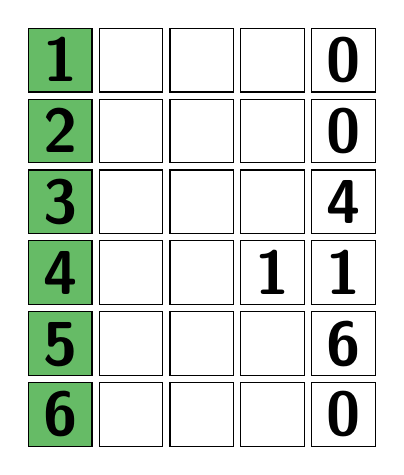
\begin{tikzpicture}[every node/.style={draw, black, text=black, font=\bfseries\sffamily\Huge, minimum size=.90cm}, scale=0.9, transform shape]
				\node [fill=CORRECT] at (0,0) {1};
				\node [] at (1,0) {};
				\node [] at (2,0) {};
				\node [] at (3,0) {};
				\node [] at (4,0) {0};

				\node [fill=CORRECT] at (0,-1) {2};
				\node []			 at (1,-1) {};
				\node [] 			 at (2,-1) {};
				\node [] 			 at (3,-1) {};
				\node [] 			 at (4,-1) {0};

				\node [fill=CORRECT] at (0,-2) {3};
				\node []			 at (1,-2) {};
				\node [] 			 at (2,-2) {};
				\node [] 			 at (3,-2) {};
				\node [] 			 at (4,-2) {4};

				\node [fill=CORRECT] at (0,-3) {4};
				\node []			 at (1,-3) {};
				\node [] 			 at (2,-3) {};
				\node [] 			 at (3,-3) {1};
				\node [] 			 at (4,-3) {1};

				\node [fill=CORRECT] at (0,-4) {5};
				\node []			 at (1,-4) {};
				\node [] 			 at (2,-4) {};
				\node [] 			 at (3,-4) {};
				\node [] 			 at (4,-4) {6};

				\node [fill=CORRECT] at (0,-5) {6};
				\node []			 at (1,-5) {};
				\node [] 			 at (2,-5) {};
				\node [] 			 at (3,-5) {};
				\node [] 			 at (4,-5) {0};
			\end{tikzpicture}
			
		\end{center}
\end{itemize}

\end{document}
